\documentclass{article}
\usepackage{amsmath}
\usepackage{amssymb}
\usepackage{graphicx}
\usepackage{hyperref}
\usepackage[version=4]{mhchem}


\begin{document}
Let \(M\) be the midpoint of side \(A B\) of triangle \(A B C\). Let \(P\) be a point on \(A B\) between \(A\) and \(M\), and let \(M D\) be drawn parallel to \(P C\) and intersecting \(B C\) at \(D\). If the ratio of the area of triangle \(B P D\) to that of triangle \(A B C\) is denoted by \(r\), then\\
(A) \(\frac{1}{2}<r<1\) depending upon the position of \(P\)\\
(B) \(r=\frac{1}{2}\) independent of the position of \(P\)\\
(C) \(\frac{1}{2} \leq r<1\) depending upon the position of \(P\)\\
\centering
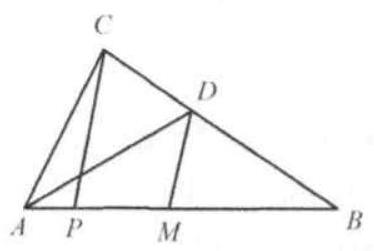
\includegraphics[width=\textwidth]{images/014(1).jpg}\\
(D) \(\frac{1}{3}<r<\frac{2}{3}\) depending upon the position of \(P\)\\
(E) \(r=\frac{1}{3}\) independent of the position of \(P\)

Solution: (B).\\
Let \(r=\frac{S_{\triangle B P D}}{S_{\triangle A B C}}\)\\
Draw the median \(C M\). Connect \(D P\). Let the intersection point be \(N\).\\
Since \(P C / / M D, S_{\triangle C D N}=S_{\triangle M P N}\).\\
Thus \(S_{\triangle B P D}=S_{\triangle B C M}\)\\
\centering
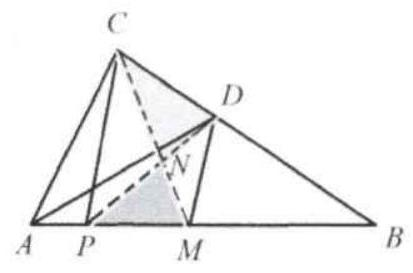
\includegraphics[width=\textwidth]{images/014.jpg}

Since \(C M\) is the median, \(S_{\triangle B P D}=S_{\triangle B C M}=\frac{1}{2} S_{\triangle A B C}\)\\
Substituting (2) into (1): \(r=\frac{S_{\triangle B P D}}{S_{\triangle A B C}}=\frac{1}{2}\).
\end{document}
